\documentclass[xcolor=svgnames]{beamer}
% Without an option, colors available are from the 15-color xcolor palette.
% xcolor=dvipsnames gives 68 options, and xcolor=svgnames has 147,
% with progressively fruitier names.

\usecolortheme[named=FireBrick]{structure}
% Could also define a color as A!n!B to make a blend that is n% A and the rest B.
% Also, [RGB={a,b,c}] is an option for a custom color.

\usepackage{amssymb}
\usepackage{textcomp}
\usepackage{wasysym}
\usepackage{listings}

\usetheme{CambridgeUS}
\usecolortheme{beaver}
\useoutertheme{infolines}
\useinnertheme{circles}
\usefonttheme{structuresmallcapsserif}
% Complete set of themes and "color themes" with snapshots: http://www.hartwork.org/beamer-theme-matrix/
%
% rows of that matrix are themes for use with \usetheme{xxx} such as:
% AnnArbor, Antibes, Bergen, Berkeley, Berlin, Boadilla, CambridgeUS, Copenhagen, Darmstadt, default, Dresden, 
% Frankfurt, Goettingen, Hannover, Ilmenau, JuanLesPins, Luebeck, Madrid, Malmoe, Marburg, Montpellier, 
% PaloAlto, Pittsburgh, Rochester, Singapore, Szeged, Warsaw
%
% columns are "color themes" for complementary use with \usecolortheme{xxx} such as:
% albatross, beaver, beetle, crane, default, dolphin, dove, fly, lily, orchid, rose, seagull, seahorse, whale, wolverine
%
% see also "inner themes" (\useinnertheme{xxx}), which dictate how to format title pages, 
% itemize/enumerate/description lists, theorem/proof environments, 
% figures, tables, footnotes, and references:
% default, circles, rectangles, rounded, inmargin
%
% "outer themes" (\useoutertheme{xxx}), which dictate head- and footline, sidebars, logo, and frame title:
% default, infolines, miniframes, smoothbars, sidebar, split, shadow, tree, smoothtree
%
% and "font themes" (\usefonttheme{xxx}):
% default, professionalfonts, structurebold, structureitalicserif, structuresmallcapsserif
%
% Full list of options and examples for all kinds of themes in beamer user guide.

% Other examples of the millions of things you can do:
\setbeamertemplate{items}[circle]
\setbeamertemplate{blocks}[rounded][shadow=false]
\setbeamertemplate{navigation symbols}{}
\setbeamercovered{dynamic}

%\setbeamercolor{title}{fg=PapayaWhip}
%\setbeamercolor{normal text}{bg=BurlyWood,fg=WhiteSmoke}

% Title page info
\title[MSRI HOPS]{HOPS code outline}
\subtitle[]{MSRI}
\author[J. Barrett ]{John Barrett}
\institute[MIT]{Massachusetts Institute of Technology}
\date[10/5/2020]{10/5/2020}

%\newtheorem{goal}{Goal}


\begin{document}


\section{Outline}

\begin{frame}{Basic Architecture}

\begin{center}
      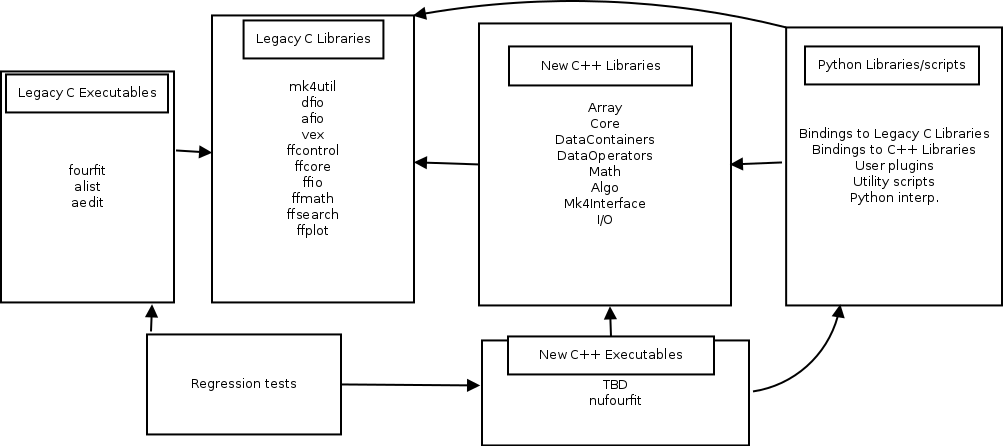
\includegraphics[width=\textwidth]{arch_overview.png}\\
\end{center}

\end{frame}

\begin{frame}[fragile]{C++ (Meta) Data Containers}

\begin{lstlisting}[language=C++,basicstyle=\ttfamily\tiny,keywordstyle=\color{red}]
template <typename XKeyType, typename... XValueTypeS>
class HkMultiTypeMap;
\end{lstlisting}

\begin{itemize}
\item Template class HkMultiTypeMap - allows for dynamic storage of different types in a single object (types must be known at compile type)
\item Accessible via a single key type (int, string, etc.)
\item Example use case: labelling axes with information that may only be known at run-time
\item Similar in behavior to a python dict(), however the number of types is limited (configured at compile time) and the desired type
must be known at the time of retrieval
\item Much more flexible than static c-structs, memory foot print is not fixed.
\end{itemize}
 
\end{frame}

\begin{frame}[fragile]{C++ Data Containers}

\begin{lstlisting}[language=C++,basicstyle=\ttfamily\tiny,keywordstyle=\color{red}]
template< typename XValueType, std::size_t RANK> 
class HkArrayWrapper
\end{lstlisting}

\begin{itemize}
\item Most large data objects inhert from another template class - HkArrayWrapper
\item This provides and interface to wrap a large multi-dimensional array.
\item The number of dimensions (rank) of the array must be known at compile time and is a template parameter
\item Responsible for handling memory management, but can provide access to pointer to raw underlying memory
\item Provides convenience functions, such resize(), and 'matrix' style-notation access via operator(i,j,...n)
\end{itemize}

\end{frame}

\begin{frame}[fragile]{C++ Data Containers}

\begin{lstlisting}[language=C++,basicstyle=\ttfamily\tiny,keywordstyle=\color{red}]
template< typename XValueType >
class HkVectorContainer: public HkArrayWrapper< XValueType, 1>, public HkNamed
\end{lstlisting}

\begin{itemize}
\item Template class HkVectorContainer
\item Provides interface for simple 1-D array of data
\item Primary use-case is for a single coordinate axis associated with a multi-dimensional array
\item For example; What are the frequencies associated with the data indexed at i=0, 1, 4,...n?
\end{itemize}

\end{frame}


\begin{frame}[fragile]{C++ Data Containers}

\begin{lstlisting}[language=C++,basicstyle=\ttfamily\tiny,keywordstyle=\color{red}]
template< typename...XAxisTypeS >
class HkAxisPack:  public std::tuple< XAxisTypeS... >
\end{lstlisting}

\begin{itemize}
\item Template class HkAxisPack
\item This is essentially a 'tuple' of HkVectorContainer, each one associated with the coordinate axis of each dimension of a multidimensional data array (HkTensorContainer)
\item Also allows for intervals of the array (along a particular axis) to be tagged with meta-data, e.g. data from [4,9) is channel:'b'.
\item Meta data tagging is done via an HkAxisLabel (which consists of an interval [a,b) along with a HkMultiTypeMap to store key:value pairs).
\end{itemize}

\end{frame}

\begin{frame}[fragile]{C++ Data Containers}

\begin{lstlisting}[language=C++,basicstyle=\ttfamily\tiny,keywordstyle=\color{red}]
template< typename XValueType, typename XAxisPackType >
class HkTensorContainer: 
public HkArrayWrapper< XValueType, XAxisPackType::RANK::value>, 
public XAxisPackType, public HkNamed
\end{lstlisting}

\begin{itemize}
\item Template class HkTensorContainer
\item Provides the interface to a multi-dimensional array of data (of a single type) long with the coordinate axis of each dimension.
\item Main use-case is the storage of correlated visibility data, but any other data which needs to be labelled with one or more coordinate axes can be stored in this class
\item For example for a single baseline - the coordinates axis of a block of visibility data (std::complex$<$double$>$) might be labelled by (time, frequency, and polarization-product).
\end{itemize}

\end{frame}


\begin{frame}{C++ Data Operators}

\begin{itemize}
\item Operators which modify data in a HkTensorContainer all derive from a uniform interface, HkArrayOperator with two virtual functions: Initialize() and ExecuteOperation()
\item Concrete data operators derive in turn from HkUnaryArrayOperator (single input/output) or HkBinaryArrayOperator (two inputs, single output).
\item New specialized operation can be defined in derived classes and composed in series, for example...(1) apply p-cal, (2) flag RFI, (3) fit single-band-delay, etc.
\item This allows them to be inserted in a list (configured at run time) so that they can be applied to the data in a user-specified way
\item Could even create a data operator which calls the python interpreter to execute user defined 'plugin' code for additional flexibility.
\end{itemize}

\end{frame}

\begin{frame}{Near term work plan}
 
 \begin{itemize}
  \item Continue getting build-system in place
  \item Add testing framework - once original HOPS programs compile we can import the existing regression tests, add integration tests for new code as available
  \item Firm-up data container types and data operator base classes
  \item Explore possibility of run-time units tracking (e.g. m, Hz, etc.) to be associated with each data container
  \item Complete Mk4-types I/O import into new data containers (test completeness with mk4 $\rightarrow$ native $\rightarrow$ mk4 conversion)
  \item I/O from DiFX into native format
 \end{itemize}

 
\end{frame}

\begin{frame}{Fourfit libraries}

\begin{center}
      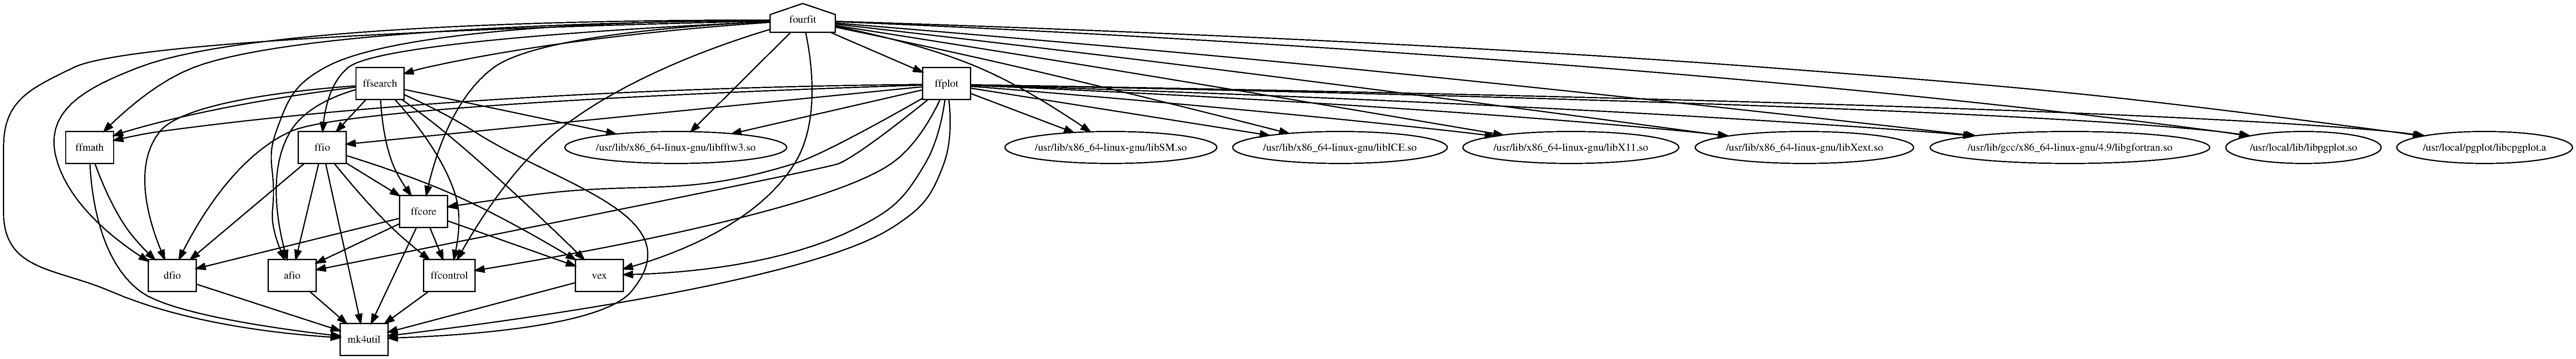
\includegraphics[width=\textwidth]{fourfit.png}\\
\end{center}

\end{frame}

\begin{frame}{ffsearch}

\begin{center}
      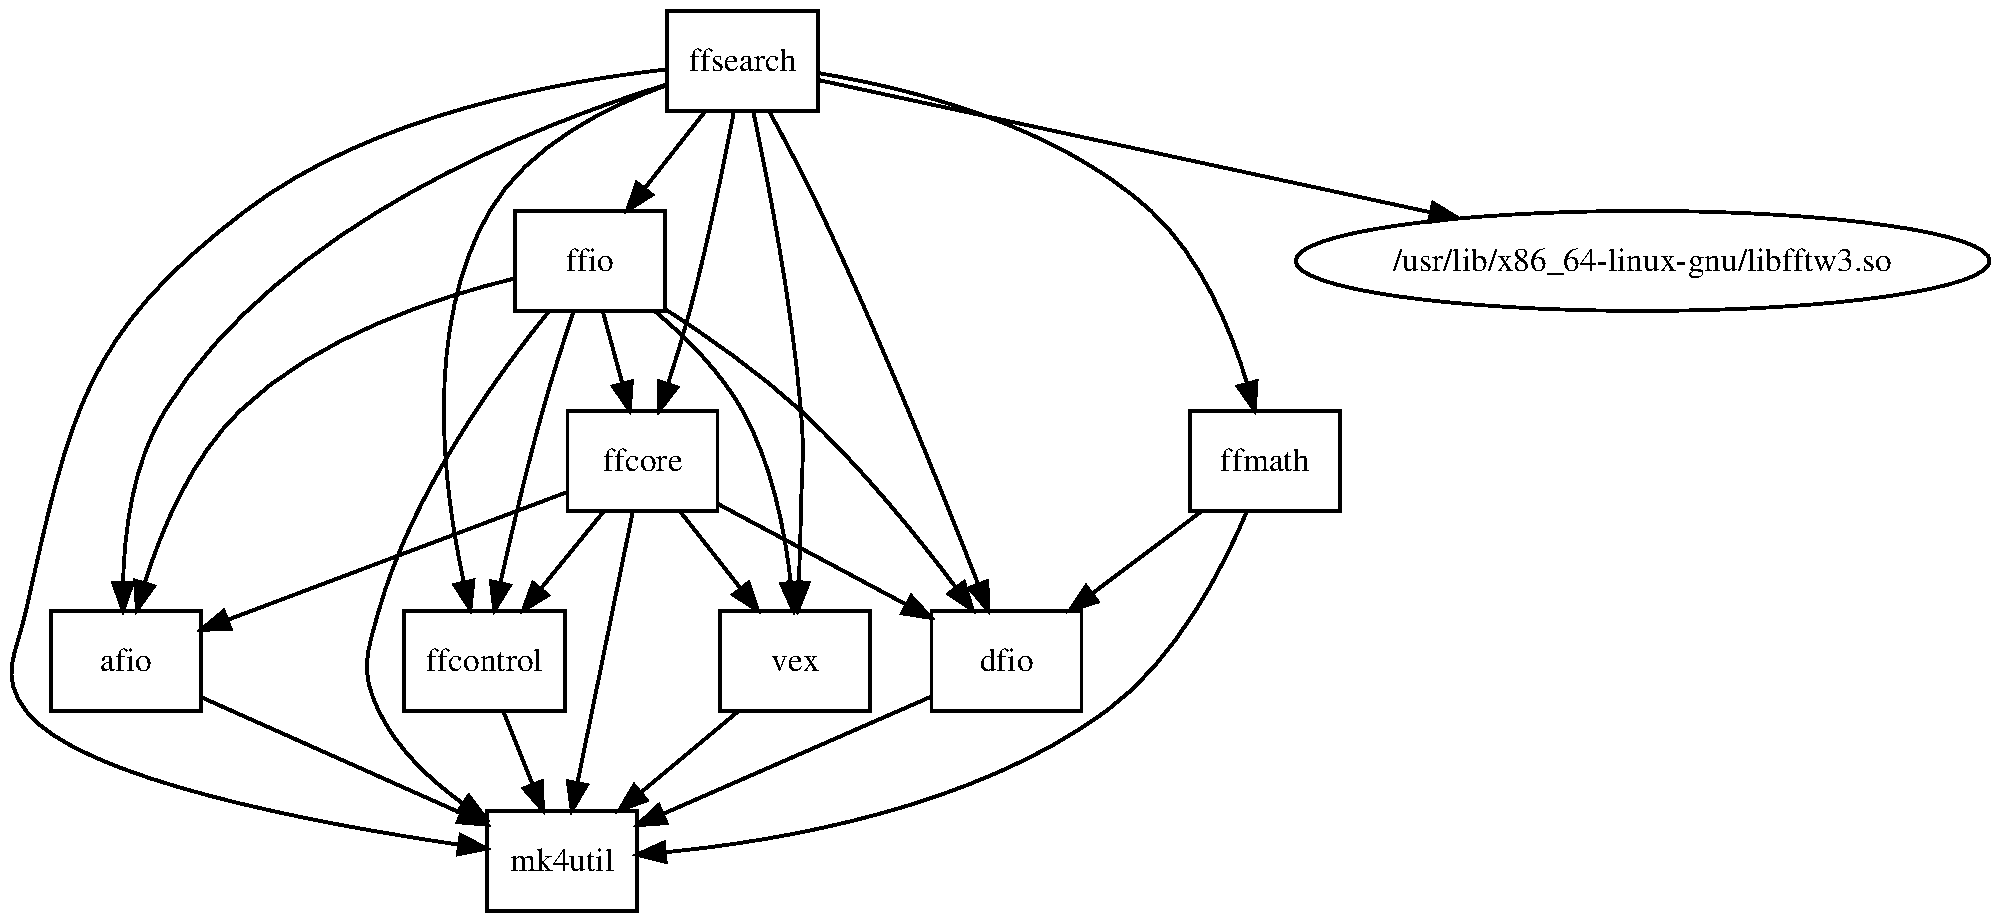
\includegraphics[width=\textwidth]{ffsearch.png}\\
\end{center}

\end{frame}




\end{document}
